\chapter{Introduction}\label{chapter:Intro}

\section{Outline}

This project aims to understand how Turing Completeness is demonstrated across different disciplines and apply them to a novel programming language, Proteus.
The goal of this thesis is to show Proteus is Turing Complete.
As such, I will first describe some major concepts such as Turing Machines, Turing Completeness, and major theorems that will be utilized.
I will supplement this with some programming language design details which prove important for showing that Proteus is Turing Complete.
Afterwards, I will describe Proteus in detail.

The following chapter will describe the different approaches from each domain showing Turing Completeness.
These include Computer Engineering, Computer Science, and Mathematics where the different proofs will be discussed in detail.

With this understanding of showing a system is Turing Complete, I will outline a proof to show that Proteus is Turing Complete.
With the proof outlined, I will discuss the design and approach.
After this, I will follow the outline to flesh out the proof.

After demonstrating that Proteus is Turing Complete, I will reflect on the knowledge gained and applied towards this project.
I will remark on some points of improvement, and then conclude the Thesis.

\section{Turing Machines}\label{sec:TM}

Alan Turing is generally considered the father of computer science for his numerous contributions including: formalization of computation theory, algorithm design, complexity theory, as well as creating the idea of the Turing Machine.
A Turing machine can be described as a machine/automata that is capable of performing operations towards some desired goal given an input.
In a sense, it was designed to be capable of performing any single computable task, such as addition, division, concatenating strings, rendering graphics, etc. \cite{TTTTM}.
TMs are at the highest level of computational power, i.e. capable of handling any computation \cite{ShallityAutomataThy}.

There are two different kinds of TMs: Deterministic and Non-deterministic.
Regardless of such a construction, both are equivalent in power to each other, and as such remain interchangeable until practice \cite{NDTMeqDTM}.
Assume all TMs discussed are Deterministic unless otherwise stated.

Figure \ref{fig:TM} is an example of a Turing Machine designed using JFLAP, see the \href{https://www.jflap.org/}{official website for JFLAP} for more information on this software (\href{https://www.jflap.org/}{https://www.jflap.org/}).
In fact JFLAP has been tested to grade students homework on computation \cite{JFLAPGrading}, showcasing just how useful this tool is.
The described machine takes an input string of 1's followed by a 0.
The machine then outputs whether there is an even number of 1's or not.
We will revisit this exact machine later in section \ref{sec:CompSci}.

\begin{figure}[htb]
    \centering
    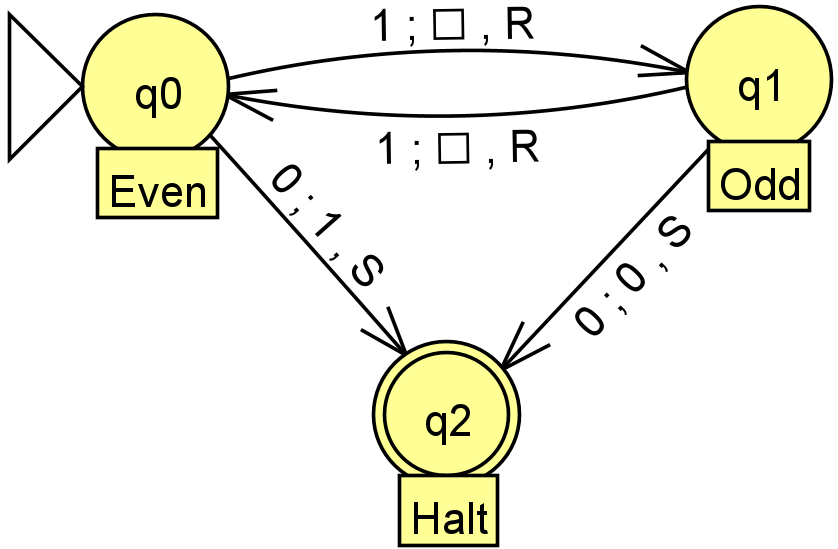
\includegraphics[width=10cm]{Images/SampleTMCrop.png}
       \caption{A TM that determines the cardinality of the length of a sequence of 1's on the tape.}
           \label{fig:TM}
\end{figure}

\subsection{Oracles}\label{subsec:Oracles}

Of course there also exists the Oracle, sometimes called Turing Machines with an oracle, which is capable of solving problems that TMs cannot.
It does so by having the ability to respond to any given problem from the TM it is connected to.
For example, the oracle would be able to solve the Halting Problem for the associated Turing Machine, but not the Halting Problem in general for all Turing Machines.
The reason the oracle is not considered more powerful is because in practice (i.e. reality), is because there is no such all-knowing source to retrieve information from.
As a result, I will disregard the Oracles for the rest of the thesis.

\subsection{Universal Turing Machines}\label{subsec:UTM}

A simple abstraction of the standard TM is a Universal Turing Machine. A UTM is capable of solving any computable problem, given the exact process/rules of the TM that will solve it.
In essence it is a machine that is not hard-coded with what to perform when given input.
The UTM will read the input, and respond based on the rules given.
As a result, the UTM is equivalently as powerful as a TM.
The only functional difference is the usability of the UTM towards a larger number of problems as opposed to the TM being created for a singular problem.

\subsection{The Church-Turing Thesis}\label{subsec:Church-Turing Thesis}

According to the Church-Turing Thesis, every effectively calculable function can be computed by a Turing Machine.
As explained by Robin Gandy, the main idea was to show that there is an upper bound on the computation of TMs.
This upper bound does not exist for humans and is therefore the basis of separation between computation power of TMs and humans.

\begin{thm}
    \label{thm:CTT}
    (Church-Turing Thesis) Every effectively calculable function can be computed by a Turing Machine.
\end{thm}

He proposed a series of four Principles that we still use today as a basis for determining what one of the definitions of a TM is capable of computing.
Any automata that violates any of these Principles is said to have "free will", which in context means being able to compute any non-computable function.
As an example, the Oracle machine would be capable of computing a non-computable function, namely the halting problem, and thus would have "free will".
We disregard such automata as there aren't any systems that exist in reality as of yet to display "free will".
As a result, TMs are the most powerful automata that can compute any calculable function.
This is why the Church-Turing thesis is generally assumed to be true \cite{GandyPaper}.

\subsection{Rice's Theorem}\label{subsec:RiceThm}

Another famous theorem to consider is Rice's Theorem.
It is widely known in the domain of computability theory as it defines the bounds of research in a formal manner.
Below is the Formal statement of Rice's Theorem, which will be supplemented with a concise statement summarizing the theorem \cite{WolframRiceThm,WikiRiceThm}.

\begin{thm}
    \label{thm:RiceThm}
    (Rice's Theorem) Let $\varphi$ be an admissable numbering of partial computable functions. 
    Let P be a subset of $\mathbb{Z}$.
    Suppose that:
    \begin{enumerate}
        \item P is non-trivial: P is neither empty nor $\mathbb{N}$ itself.
        \item P is extensional: $\forall  m,n \in \mathbb{N}$, if $\varphi_{m} = \varphi_{n}$,
        then $m \in P \Leftrightarrow n \in P$.
    \end{enumerate}
    Then P is undecidable.

    I.e. The only decidable index sets are $\emptyset$ and $\mathbb{N}$.
\end{thm}

This directly translates to programming languages as stating: All non-trivial smenatic properties of programs are undecidable.
Thus, Rice's theorem is a generalization of the Halting Problem.
Because of this theorem, it is impossible to design a program that determines if a given program is able to execute without error.
Another view of thie theorem is that it states only trivial properties of programs are algorithmically decidable.
Eg. If a program has an if statement inside the code.

\section{Turing Completeness}\label{sec:TC}

Turing Completeness is a closely related term when discussing Turing Machines.
For a system to be Turing Complete, it must be capable of performing any computation that a standard TM can perform.
An equivalent description would be that for a system to be TC, it must simulate a UTM.
By transitivity, if any system is proven to be TC, then it must be equivalent in power to all other systems that are TC.
Therefore, all TC systems are considered the most powerful computation machine.

\subsection{Considering the Practicality of Turing Complete Programming Languages}\label{subsec:PracticalTC}

Despite all TC systems being equivalent in computation power, this does not mean that all are practically useful.
This is because despite the TC being able to simulate any TM, it may have a more complex method for simulation or calculation of the same problem.
This is considered a non-issue as the length of time needed for computation is not considered when discussing TMs and TC systems.
This is only a factor for practical purposes, such as programming languages, space and time complexity are of major importance.

\subsubsection{Esoteric Progamming Languages}\label{subsubsec:EsotericPL}

Esoteric programming languages are designed to demonstrate a key concept with language design, but are often done so in a joking manner.
An example of a highly simplistic well-known esoteric TC language is brainfuck.
I will describe the way brainfuck operates and then provide several example programs with explanations.

The language has only 8 instructions, a data pointer, and an instruction pointer.
It uses a single dimensional array containing 30,000 byte cells, with each cell initialized to zero.
The data pointer points to the current cell within the array, initialized to index 0.
The instruction pointer points to the next instruction to be processed, starting from the first character given in the code.
Any characters besides those used in the instructions are considered comments and will be ignored.
Instructions are executed sequentially unless branching logic is taken via the '[' or ']' instructions.
The program terminates when the instruction pointer moves beyond the final command.
Additionally, it has two streams of bytes for input and output which are used for entering keyboard input and displaying output on a monitor using the ASCII encoding scheme \cite{BfWiki,BfGH}.

The 8 instructions are as follows:
\begin{table}[h!tb]
    \centering
    \begin{tabular}{|c|p{10cm}|}
        \hline
        \textbf{$>$} & Increments the data pointer by one. (This points to the next cell on the right). \\
        \hline
        \textbf{$<$} & Decrement the data pointer by one. (This points to the next cell on the left). \\
        \hline
        \textbf{$+$} & Increments the byte at the data pointer by one. \\
        \hline
        \textbf{$-$} & Decrements the byte at the data pointer by one. \\
        \hline
        \textbf{$.$} & Output the byte at the data pointer. \\
        \hline
        \textbf{$,$} & Accept one byte of input, storing its value in the byte at the data pointer.\\
        \hline
        \textbf{[} & If the byte at the data pointer is zero, then instead of moving the instruction forward to the next command, go to the matching ']' command. (Jump forwards). \\
        \hline
        \textbf{]} & If the byte at the data pointer is non-zero, then instead of moving the instruction forward to the next command, go to the matching '[' command. (Jump backwards). \\
        \hline
    \end{tabular}
    \caption{Brainfuck Instruction Set}
    \label{tab:BrainfuckInstructionSet}
\end{table}

Each '[' or ']' must correspond to match with it's complement symbol, namely ']' and '[' respectively.
Also, when input is read with the ',' command the given character from a keyboard input will have its value read as a decimal ASCII code
(eg. '!' corresponds to 33. 'a' corresponds to 97, etc.).
The decimal value is what is then converted to binary and stored within the current byte \cite{BfSO}.

Here is a simple program that modifies the value of the first cell in the 30,000 byte array.

\begin{verbatim}
    ++      Add 2 to the byte value in cell 0
    [-]     Decrement the value of the current cell until it reaches 0
\end{verbatim}

In fact, we can remove the comments and put the code onto a single line to achieve the same result.
Recall that comments include any character that is not listed as one of the 8 aforementioned instructions.

\begin{verbatim}
    ++[-]
\end{verbatim}

\newpage

An equivalent program in python is seen below:

\begin{verbatim}
    # Let 'Array' be our 30,000 byte array
    Array[0] += 2
    while (Array[0] != 0):
        Array[0] -= 1
\end{verbatim}

Below is an example program that outputs Hello World.
At the end of each line is the end result of the operations done in the line as a comment.
Each line prints a new character.

\begin{verbatim}
    >++++++++[<+++++++++>-]<.       H
    >++++[<+++++++>-]<+.            e
    +++++++..                       l
    +++.                            l
    >>++++++[<+++++++>-]<++.        o
    ------------.                   [space]
    >++++++[<+++++++++>-]<+.        W
    <.                              o
    +++.                            r
    ------.                         l
    --------.                       d
    >>>++++[<++++++++>-]<+.         !
\end{verbatim}

For an in-depth breakdown of brainfuck with examples and guiding logic like the one above, read: \cite{BfGH}.
One common technique utilized when creating programming languages is to bootstrap them.
This means that the developers will write a compiler for the language, using the language itself.
This is done for many reasons, but the reason for introducing it here is to show how brainfuck is capable of complex logic that is more practically useful than simple programs as seen above.
Below is the current smallest bootstrapped compiler for brainfuck \cite{SmallestBfCompiler,SmallestBfCompilerActual}.

\begin{verbatim}
    >>>+[[-]>>[-]++>+>+++++++[<++++>>++<-]++>>+>+>+++++[>++>++++++<<-]+>>>,
    <++[[>[->>]<[>>]<<-]<[<]<+>>[>]>[<+>-[[<+>-]>]<[[[-]<]++<-[<+++++++++>[
    <->-]>>]>>]]<<]<]<[[<]>[[>]>>[>>]+[<<]<[<]<+>>-]>[>]+[->>]<<<<[[<<]<[<]
    +<<[+>+<<-[>-->+<<-[>+<[>>+<<-]]]>[<+>-]<]++>>-->[>]>>[>>]]<<[>>+<[[<]
    <]>[[<<]<[<]+[-<+>>-[<<+>++>-[<->[<<+>>-]]]<[>+<-]>]>[>]>]>[>>]>>]<<[>>
    +>>+>>]<<[->>>>>>>>]<<[>.>>>>>>>]<<[>->>>>>]<<[>,>>>]<<[>+>]<<[+<<]<]
\end{verbatim}

As we quickly found out, using brainfuck in any practical sense is simply too much work due to its extreme inefficiency.
It also is extremely difficult to understand without comments indicating the goal of each step.
Due to the simplicity of the language, it is very useful for studying Turing Completeness.
There exist many other esoteric TC programming languages, but the reason for choosing brainfuck in particular is its simple instruction set.
As a result, we will now look at more useful and practical programming language paradigms.
These languages within these paradigms will be much more efficient and legible, at the cost of increased complexity in instruction set.

\subsubsection{Procedural Languages}\label{subsubsec:PL}

Procedural Programming Languages are designed to be read linearly in execution order, top to bottom.
The main idea behind this design of languages is to create procedures and subprocedures (equivalently routines and subroutines), to achieve a larger goal.
For example to calculate the sum of squares in code you may design it in the C code as follows:

\begin{verbatim}
    float squareNumber(float a) {
        return a * a;
    }
    float findSumOfSquares (float a, float b) {
        return squareNumber(a) + squareNumber(b);
    }
\end{verbatim}
    
When working in Procedural Programming Languages, variables are used to store and modify data.
These variables may be locally or globally defined, which is where we define the concept of scope.
Scope refers to the current lens in which we view code and the system memory.
It identifies which variables exist, what values they have, and what operations are being performed.
The below example in C provides insight into the importance of scope.

\begin{verbatim}
    float globalVariable;

    float foo (float bar) {
        float localVariable;
        ...
    }

    float baz (float qux) {
        float localVariable;
        ...
    }
\end{verbatim}

Notice that we are able to utilize a variable named localVariable in the two functions foo and baz.
This is allowed because when the scope is inside of either function, the other function does not exist.
The variable globalVariable is available to both because it is outside of the scope of both functions.
This means that any other function in the code in the same scope as the globalVariable is capable of accessing its value.

I will now describe the importance of functions in Procedural Programming Languages.
Functions are designed to complete a single goal and return a single output.
They are capable of accepting a non-negative number of inputs and outputting 0 or 1 outputs.
These functions are capable of calling other functions, including themselves.
When a function calls itself, this is called recursion.
Here is an example constructing the fibonacci sequence in C in 2 ways: without recursion, and with recursion.

\begin{verbatim}
    //Given an integer n, calculate the first n numbers
    //of the fibonacci sequence without recursion
    
    void sequentialFibonacci (int n) {
        if (n < 1) {
            printf("Input must be an integer greater than 0");
                return;
        }

        int sub1 = 0;
        int sub2 = 1;

        for (int i = 1; i <= n; i+=1) {
            if (i > 2) {
                int curr = sub1 + sub2;
                sub1 = sub2;
                sub2 = curr;
                printf("%d ", curr);
            }
            else if (i == 1) {
                printf("%d ", sub1);
            }
            else if (i == 2) {
                printf("%d ", sub2);
            }
        }
    }

    /***************************************************************/

    //Recursive case

    //keep track of current Index, given amount of fibonacci numbers
    //to print, and propogate the two subnumbers to the next step
    void recursiveFibonacci (int currIndex, int n, int sub1, int sub2) {
        if (currIndex < n) {
            printf("%d ", sub1 + sub2);
            recursiveFibonacci(currIndex + 1, n, sub2, sub1 + sub2);
        }
        return;
    }

    //handle base cases (exit conditions)
    //otherwise start the recursive process
    void startRecursiveFibonacci (int n) {
        if (n < 1) {
            printf("Input must be an integer greater than 0");
        } else if (n == 1) {
            printf("%d ", 0);
        } else if (n == 2) {
            printf("%d %d ", 0, 1);
        } else {
            printf("%d %d ", 0, 1);
            recursiveFibonacci(0, n - 2, 0, 1);
        }
        return;
    }
\end{verbatim}

As shown above, recursion is a powerful tool to simplify the amount of lines needed to code the main functionality of the procedure.
It simplifies the amount of lines written because the overall logical design is more complex.

Through the use of scope and compartmentalizing procedures, Procedural programming is a very straightforward and capable design paradigm for software development.
Some well known languages that are Turing Complete from this paradigm are: 
\begin{itemize}
    \item C
    \item Pascal
    \item COBOL
    \item Fortran
    \item ALGOL
    \item Basic        
\end{itemize}

Although these languages are very old, with some coming from the 1960s, some still find modern use.
Linus Torvalds, the creator of the Linux kernel and git, chose C to be the main language for developing both of these well known pieces of software.
Both are still actively developed and improved to this day and remain majorly written in C \cite{GitMadeinC,LinuxMadeinC}.
Additionally, Richard Stallman led the development for the GNU operating system using C \cite{GNUPreferC}.
Although most users are on the Windows or Apple platform for PCs, the GNU operating system with the Linux kernel is still a popular choice amongst users looking for a different experience \cite{MarketShareOS}.
Besides C, COBOL remains a language that is used professionally for banking.
Many banks still use COBOL their business application and management \cite{COBOLBanks}.

\subsubsection{Object Oriented Languages}\label{subsubsec:OOPL}

A different scheme altogether for a programming language is an Object Oriented Language.
Developing in this language paradigm is known as a Object Oriented Programming.
OOP is structured entirely different than Procedural Programming.
Instead of defining procedures to solve the problem, we utilize a new idea of coding.
We outline classes, which are representations of some system that we wish to design.
Classes contain 3 parts: Data Members, Constructors, and Methods.
Data Members are used to describe what the Class is.
For example, if I want to model a school, an important data member would be the amount of students enrolled.
Constructors are ways to create an instance of the class.
This is where the object is created.
In the school example, perhaps there would be two ways to create a school: with a total amount of students enrolled already, and another without.
Both are valid as adding an existing school to the digital system would use the first constructor, while creating a new school would utilize the second constructor.
Methods are ways we modify the attributes of the objects.
Perhaps a certain amount of students enroll into the newly created school.
We must have a way to update the amount of students for any school.
These 3 parts form the basis of what OOP looks like.
Below is a snippet of Java code demonstrating these principles.

\begin{verbatim}
class School {
    private int numEnrolledStudents;
    
    public School () {
        this.numEnrolledStudents = 0;
    }
    
    public School (int numAlreadyEnrolled) {
        this.numEnrolledStudents = numAlreadyEnrolled;
    }
    
    public int getNumEnrolled() {
        return this.numEnrolledStudents;
    }
    
    public void setNumEnrolled(int numStudents) {
        this.numEnrolledStudents = numStudents;
        return;
    }
}

class RunCode {
    public static void main(String[] args) {
        School NewSchool = new School();
        
        System.out.println("The number of students enrolled 
            in the new school is: " + NewSchool.getNumEnrolled()); // 0
        
        NewSchool.setNumEnrolled(100);
        
        System.out.println("The number of students enrolled
            in the new school is: " + NewSchool.getNumEnrolled()); // 100
        
        School CSUN = new School(32172);
        
        System.out.println("The number of students enrolled
            at CSUN is: " + CSUN.getNumEnrolled());                // 32172
    }
}
\end{verbatim}

There are more advanced features such as Inheritance that allow for more complex design models.
Furthermore, Java contains Modifiers which are used to change the permission of which piece of code is capable of being accessed by another piece of code.
In the above example, only the school object is capable of managing the data of numEnrolledStudents \cite{CSUNStudents}.
Through the use of the methods getNumEnrolled and setNumEnrolled, any other class can modify the value of the class, but only through the reference of the school object.

Some well known languages that are Turing Complete from this paradigm are: 
\begin{itemize}
    \item Java
    \item C++
    \item Scala
    \item PHP
    \item Perl
    \item Swift        
\end{itemize}

Java is utilized today for a variety of applications including: embedded systems, android mobile apps, and web-apps \cite{JavaUse1, JavaUse2}.
PHP is a language that is mostly used for web development.
It is primarily used as a scripting language for servers \cite{PHPScriptingServer}.
It's most commonly seen in the Laravel framework as well as for WordPress \cite{PHPLaravel,PHPWP}.
C++ also sees a wide variety of applications that it's used for.
Some things include OSs like Microsoft Windows and Linux \cite{CPPUse1,CPPUse2}.
Firefox, an open source browser, is also made using C++ \cite{CPPFirefox,FirefoxMain}.
Java, PHP, and C++ remain some of the most desired languages for jobs in the market today \cite{TopLangs1,TopLangs2,TopLangs3}.

\subsubsection{Multi Paradigm Languages}\label{subsubsec:MultiParadigmPL}

Some languages allow for the combination of OOP and Procedural Programming.
In such paradigms, the code allows for both to be run at the same time and enjoys the benefits of both approaches, at the cost of increased design overhead of the project.
The most desired languages today are Python and Javascript due to their simplicity and numerous list of libraries to code just about any project of any scale \cite{EasyLangs1,EasyLangs2,PyLibs,NPM,Yarn}.
Such languages are amongst the most desired as well today \cite{TopLangs1,TopLangs2,TopLangs3}.

Here is an example snippet of Python code that demonstrates both object oriented and procedural programming at the same time:

\begin{verbatim}
    # Sequential Programming
    def findSumOfSquares(num1, num2):
        return (num1 ** 2) + (num2 ** 2)

    # OOP
    class Homework:
        def __init__(self, problem):
            self.problem = problem
            
        def problem(self, problem):
            self.problem = problem

    # Creating the 'Homework' object and printing a method from it
    HW = Homework("What is the sum of squares of 2 and 3?")
    print(HW.problem)

    # Utilizing a function created from sequential programming
    print(findSumOfSquares(2, 3))




    #####       Printed to Terminal     #####

    What is the sum of squares of 2 and 3?
    13
\end{verbatim}

In the code example, we utilize Procedural Programming to create the findSumOfSquares function.
Through the usage of OOP, we create a Homework object that has a single data member, a single problem.
By accessing the problem within the Homework object, we are able to print it out, then use the function to solve it.

Some well known languages that are Turing Complete from this paradigm are shown below.
Notice that some languages mentioned in the previous sections may show up in the list: 
\begin{itemize}
    \item JavaScript
    \item C++
    \item Python
    \item R
    \item Perl
    \item Fortran
\end{itemize}

Multi Paradigm languages have a lot of flexibility for the applications that they can be used to create.
The top frontend frameworks for web development use Javascript as their main language including React, Vue, Svelte, and more \cite{JSPopular}.
Python is very popular for its legible and flexible code.
With its libraries such as Tensorflow and Keras, Machine Learning and other AI subgenres are easier to implement than in other languages.
The popular LLM ChatGPT is primarily written in python \cite{ChatGPTPython}.
R is another language that is popular for its data science capabilities.
It is heavily used within the sciences (alongside python) because of its simplistic syntax, as well as its numerous libraries for data analysis \cite{RDataSci,DataSciLangs}.

%%%%%%%%%%%%%%%%%%%%%%%%%%%%%%%%%%%%%%%%%%%%%%%%%%%%%%%%%%%%%%%%%%%%%%%%%%%%%%%%%%%%%%%%%%%%%%%%

\subsubsection{Functional Programming Languages}\label{subsubsec:FPL}

Functional Programming Languages take an entirely different approach to coding.
These languages are based on lambda calculus and are not often taught to new programmers due to their unique style.
They usually follow a simple design of pure functions:
\begin{enumerate}
    \item Referential Transparency: The same output is produced for all arguments given
    \item Immutability: There is no modification to the arguments given, I/O streams, or local/global variables.
\end{enumerate}

FP has the unique property of being immutable for all functions and arguments \cite{FP1,FP2,RefTransp1,RefTransp2}.
FP functions also only use the arguments given for a particular task.
Below are some simplistic code examples in Haskell:

\begin{verbatim}
    -- Function to add two numbers
    addTwoNumbers :: Num a => a -> a -> a
    addTwoNumbers x y = x + y
    
    -- Function to find the square of a number
    findSquare :: Num a => a -> a
    findSquare x = x * x
    
    -- Function to find the sum of squares
    findSumOfSquares :: Num a => a -> a -> a
    findSumOfSquares x y = addTwoNumbers (findSquare x) (findSquare y)
    
    -- Main function
    main :: IO ()
    main = do
        let num1 = 2
        let num2 = 3
        let result = findSumOfSquares num1 num2
        putStrLn ("The sum of squares is: " ++ show result) 

        #####       Printed to Terminal     #####

        The sum of squares is: 13

\end{verbatim}

This looks like a more advanced version of lambda calculus seen in \ref{subsec:LambdaCalc}.
It operates by defining the function and its arguments.
Once the definition is completed, you write out the logic for the function.
One can chain these outputs like the functions in section \ref{subsubsec:PL}.
To implement loops, recursion is required.

\begin{verbatim}
    -- Function to compute the nth Fibonacci number
    fibonacci :: Integer -> Integer
    fibonacci n
        | n < 0     = error "Negative input is not allowed"
        | n == 0    = 0
        | n == 1    = 1
        | otherwise = fibonacci (n - 1) + fibonacci (n - 2)

    -- Function to generate a list of Fibonacci numbers up to the nth number
    fibonacciList :: Integer -> [Integer]
    fibonacciList n = [fibonacci x | x <- [1..n]]

    -- Main function to print Fibonacci numbers up to the nth Fibonacci number
    main :: IO ()
    main = do
        let n = 4  -- User-defined bound for Fibonacci sequence
        let fibNumbers = fibonacciList n
        putStrLn ("The first " ++ show n ++  
            " Fibonacci numbers are: " ++ show fibNumbers)

    #####       Printed to Terminal     #####

    The first 4 Fibonacci numbers are: [1,1,2,3]
\end{verbatim}

Some well known languages that are Turing Complete from this paradigm are:  
\begin{itemize}
    \item Lisp
    \item Haskell
    \item Elixir
    \item OCaml
    \item Scala
\end{itemize}

Haskell and Elixir are used by many companies as a way for writing their software \cite{HaskellList,HaskellListReadme,ElixirList,ElixirListReadme}.
They are used for a variety of purposes such as security, browsers, and more.
Coq is a proof assistant that allows users to codify their proofs and assert their findings.
Coq was developed using OCaml \cite{OCamlCoq}.
For my experience using Coq alongside some other proof assistants Dafny and TLA+, see Appendix \ref{app:ProofAssist}.

\newpage
Some benefits of using functional programming are:
\begin{itemize}
    \item Unit Testing
    \item Debugging
    \item Concurrency
\end{itemize}

Unit Testing is made easier because of the immutable property.
By not allowing for modification of items, it is easier to determine which tests fail.
Furthermore, it forces more thought to be considered when designing the program.

Debugging is also made easier for similar reasons.
Because functions are explicitly defined with inputs and ouputs with the immutability on all elements, this means that when there is an error it is simple to find.
When there is a logical error, the solution is apparent more rapidly because of the logical flow of the program.
When there is a compiler error, then instead the stack trace returns where the problem is.

Concurrency is also inherently allowed in the language because each function operates from a single thread.
This is why Erlang or Elixir is used for telecommunications from companies like CISCO or banking companies such as Goldman Sachs \cite{ErlangUses}.



\section{Proteus}\label{sec:Proteus}

The main goal of this thesis is to outline a proof demonstrating that a novel prototype language, Proteus, is TC.
In this section, I will describe in detail what Proteus is.

\subsection{Proteus Description}\label{subsec:ProteusDescription}

Proteus is a programming language and compiler being developed as a project for CSUN's Autonomy Research Center for STEAHM in collaboration with the NASA Jet Propulsion Laboratory (JPL).
JPL system engineers needed a safer language to develop autonomous systems reliably, which is why Proteus was created.
Proteus allows for the creation of different models: actors and hierarchical state machines.
It is compiled to C++ with the C++17 standard \cite{ProteusRunTime}.

Proteus is a programming language that follows the Actor model paradigm, which is somewhat related to the OOP paradigm.
The difference lies in that Actor model allows for concurrent computation, while OOP generally runs sequentially.
This means that parallelism is inherently existent in the language \cite{ActorModelParallel,ActorJavaParallel}.
Furthermore, because of the design of the events and event queue for Actors, any code involving them is run sequentially.
This means that Proteus also supports the Procedural Programming langauge paradigm.
Thus, Proteus is a Multi Paradigm language that enjoys the ability to utilize features such as scope, recursion, and so forth \cite{ProteusPaper}.

\subsubsection{Actors}\label{subsubsec:Actors}

Actors are independent entities within concurrent systems.
By allowing several actors to operate independently, there is: no sharing of resources, concurrent runtime, and only interact amongst each other via a message system.
Communication is asynchronous because the messages get buffered by the system until the recipient can handle them.
Actors can send messages, modify local state, or create more actors based on the message handling.

\subsubsection{Hierarchical State Machines}\label{subsubsec:HSM}

Hierarchical State Machines allow developers to model the system that they are developing for.
These HSMs are an extension to the standard definition of a state machine as HSMs allow states to be HSMs themselves.
This allows for simplification of the states and transitions amongst states allowing simpler models for usage in the real-world.

Actors have a non-negative amount of associated HSMs while each HSM belongs to exactly one actor.
Event Handlers are the way that messages are sent amongst machines as well as how the machine perform state transitions.
Actors and states are statically defined, which means that they cannot be created nor destroyed at runtime.
When compiled, Actors and states are created as C++ structs.

\subsection{Proteus Grammar}\label{subsec:ProteusGrammar}

Below is the Grammar for Proteus.
It outlines the command followed by the definition for writing the command.
Anything outlined in single quotations indicates text to be written explicitly.
It is to be read as: 'OPERATION' can be written as 'HOW TO WRITE THE OPERATION'.

\begin{verbatim}
Program: DefEvent* DefGlobalConst* DefFunc* DefActor+
DefActor: 'actor' ActorName '{' ActorItem* '}'
ActorItem: DefHSM | DefActorOn | DefMember | DefMethod
DefActorOn: 'on' EventMatch OnBlock
DefHSM:   'statemachine' '{' StateItem* '}'
DefState: 'state' StateName '{' StateItem* '}'
StateItem: DefOn | DefEntry | DefExit | DefMember | 
            DefMethod | DefState | InitialState
DefOn: 'on' EventMatch OnBody
EventMatch: EventName '{' [VarName (',' VarName)*] '}'
OnBody: GoStmt | OnBlock
OnBlock: Block
DefEntry: 'entry' '{' Block '}'
DefExit: 'exit' '{' Block '}'
DefMember: Type VarName '=' ConstExpr ';'
DefMethod: 'func' FuncName FormalFuncArgs ['->' Type] Block
InitialState: 'initial' StateName ';'
Block: '{' Stmt* '}'
Stmt: IfStmt | WhileStmt | DecStmt | AssignStmt | ExitStmt | 
            ApplyStmt | SendStmt | PrintStmt | PrintlnStmt
DefEvent: 'event' EventName '{' [Type (',' Type )*] }' ';'
DefFunc: 'func' FuncName FormalFuncArgs ['->' Type] Block
DefGlobalConst: 'const' Type VarName '=' ConstExpr ';'
ExitStmt: 'exit' '(' NUMBER ')' ';'
ReturnStmt: 'return' Expr ';'
DecStmt: Type VarName '=' Expr ';'
AssignStmt: VarName '=' Expr ';'
ApplyStmt: ApplyExpr ';'
SendStmt : HSMName '!' EventName ExprListCurly ';'
PrintStmt : 'print' ExprListParen ';'
PrintlnStmt : 'println' ExprListParen ';'
FormalFuncArgs : '(' [Type VarName (',' Type VarName)*] ')'
ExprListParen :'(' [Expr (',' Expr)*] ')'
ExprListCurly :'{' [Expr (',' Expr)*] '}'
Type: 'int' | 'string' | 'bool' | 'actorname' | 'statename' | 
            'eventname'
GoStmt: JustGoStmt | GoIfStmt
JustGoStmt: 'go' StateName Block
GoIfStmt: 'goif' ParenExpr StateName Block 
            ['else' (GoIfStmt | ElseGoStmt)]
ElseGoStmt: 'go' StateName Block
IfStmt: 'if' ParenExpr Block ['else' (IfStmt | Block)] 
WhileStmt: 'while' ParenExpr Block 
ParenExpr: '(' Expr ')' 
ConstExpr: IntExpr | BoolExpr | StrExpr
Expr: ValExpr | BinOpExpr | ApplyExpr
BinOpExpr: ValExpr BinOp Expr 
BinOp: '*' | '/' | '%' | '+' | '-' | '<<' | '>>' | '<' | '>' |
            '<=' | '>=' | '==' | '!=' | '^' | '&&' | '||' | '*=' | 
            '/=' | '%=' | '+=' | '-=' | '<<=' | '>>=' | '^='
ApplyExpr: FuncName ExprListParen
ValExpr: VarExpr | IntExpr | StrExpr | BoolExpr | ActorExpr | 
            StateExpr | EventExpr | ParenExpr
VarExpr: VarName
IntExpr: NUMBER 
StrExpr: STRING 
BoolExpr: BOOL
ActorExpr: 'actor' ActorName
StateExpr: 'state' StateName
EventExpr: 'event' EventName
StateName: NAME
ActorName: NAME
FuncName: NAME
VarName: NAME
EventName: NAME
\end{verbatim}

Looking at the grammar is similar to looking at the pieces of a puzzle without actually arranging the pieces together.
Below is an example written in Proteus code that showcases Actors and HSMs in a system.

There are a total of 3 events: POWER\_ON which accepts a boolean as input, POWER\_OFF, and NEXT with the latter two not accepting an inputs.
There are 2 actors: Main and Driver.
Main has a single state machine with 2 states: On and Off.
Main defines an internal boolean for whether Mode2 is enabled.
By default it is initialized to false.
The HSM within Main is initalized to Off, and switches to On when the POWER\_ON event is registered.
Furthermore, it updates the value for Mode2 being enabled with the input for POWER\_ON.
When turned On, there is a defined Mode1 that is the initial mode of the machine.
It then defines what the machine does when it is turned on and off.
In both cases, it outputs a message indicating the status of the power state of the machine (on prints on, and off prints off).
Mode1 prints to the output the current Mode, and then has logic determining what to do when the NEXT message is received.
If the machine has mode2\_enabled set to true, then it should should go to Mode2.
Mode2 simply prints the current mode when it is entered.
The second actor is the Driver.
It determines the actions to be taken by Main in a series of messages (events) that are broadcasted from its internal statemachine.
Upon turning on the machine, it will send the event for Main to turn on with an input of true.
Then it sends Main the NEXT event twice.
It then tells Main to power off with the POWER\_OFF event.

\begin{verbatim}
event POWER_ON {bool};
event POWER_OFF {};
event NEXT {};
actor Main {
    bool mode2_enabled = false;
    statemachine {
        initial Off;
        state Off {
            on POWER_ON {x} {go On {mode2_enabled = x;}}
        }
        state On {
            initial Mode1;
            entry {println(“turning on”);}
            exit {println(“turning off”);}
            on POWER_OFF {} {go Off {}}
            state Mode1 {
                entry {println(“mode 1”);}
                on NEXT {} {goif(mode2_enabled) {Mode2 {}}}
            }
            state Mode2 {
                entry {println(“mode 2”);}
            }
        }
    }
}
actor Driver {
    statemachine {
        entry {
            Main ! POWER_ON {true};
            Main ! NEXT {};
            Main ! NEXT {};
            Main ! POWER_OFF {};
        }
    }
}
\end{verbatim}

From the above example, we can see the OOP and Procedural Programming properties that Proteus is capable of.
In fact, we can see the property of scope in action.
The local variable mode2\_enabled is only accessible within Main and the HSM within Main.
Furthermore, we see that the order of events is run in sequence.
Main accepts these events in the order received in the internal event queue, and is capable of responding based on the internal state conditions as well as the event received.
When this code is run, the output is seen below:

\begin{verbatim}
    turning on
    mode1
    mode2
    mode1
    turning off
\end{verbatim}

The goal of this Thesis is to analyze this language to prove that it is TC.
This is done by looking at the grammar and type of programming paradigm.
With this understanding, we will also look at different approaches for proving Turing Completeness.
Afterwards, we will demonstrate that Proteus is in fact turing complete using some of the methods seen in the next chapter.